\chapter{Izvođenje i rezultati}
\label{chap:rezultati}

Orthobalancer je javno dostupan na URL-u
\footnotesize{\url{http://orthobalancer.bmad.bii-sg.org}}.
\normalsize

% TODO možda podijeliti ovo poglavlje na sectione (ulaz, izvođenje izlaz)

Početna stranica je prikzana na slici \ref{fig:input-html}. Pri vrhu su
smješteni HTML elementi kojima korisnik može urpavljati aplikacijom. Za odabir
načina unosa FASTA sekvence pojedinog paraloga postoje radio gumbi \engl{radio
buttons} za ručni upis, odnosno za zalijepiti sekvencu \engl{paste sequence} te
za \emph{upload} datoteke, a sama se sekvenca dodaje pritiskom na gumb \emph{Add
sequence}. Svaku sekvencu je moguće i naknadno ukloniti pritiskom na gumb
\emph{Remove} uz pojedinu sekvencu. S lijeve strane se nalaze jednostavne upute
za korištenje.

\begin{figure}[h!]
\centering
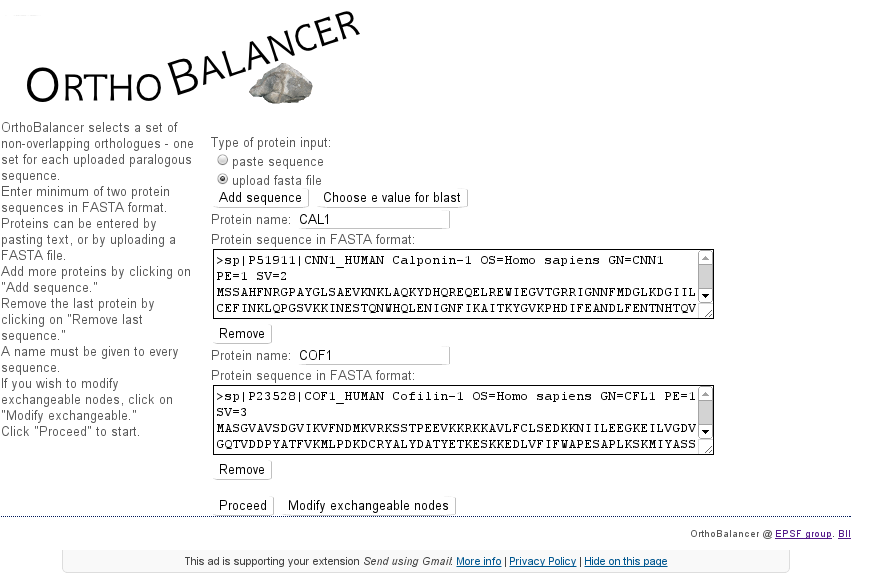
\includegraphics[width=5.8in]{figures/input-html.png}
\caption{Izgled početne stranice Orthobalancera}
\label{fig:input-html}
\end{figure} 

\begin{figure}[h!]
\centering
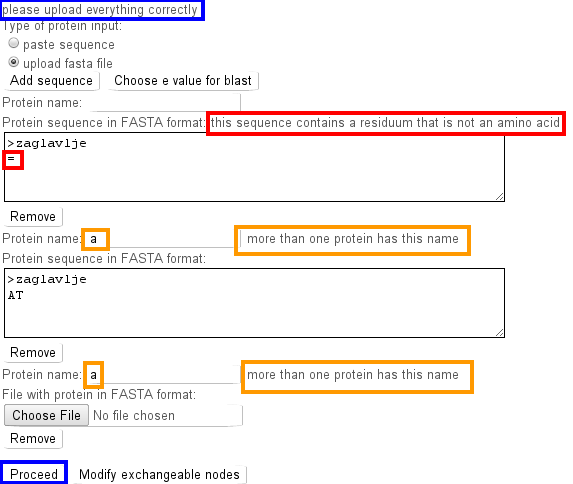
\includegraphics[width=4.8in]{figures/input-error.png}
\caption{Ponašanje početne stranice Orthobalancera}
\label{fig:input-error}
\end{figure} 
 
Sukladno s ograničenjima opisanim u odjeljku \ref{sec:input}, aplikacija je
sposobna dojaviti razne greške. Dojave grešaka označene su na slici
\ref{fig:input-error}. Narančastim okvirima označena je greška jedinstvenih
imena. Pogrešan unos FASTA sekvence označen je crvenim okvirima. Ukoliko se
pokuša pokrenuti pretraga dok su podaci pogrešni, pojavit će se upozorenje na
vrhu što je označeno plavim okvirima.

\begin{figure}[h!]
\centering
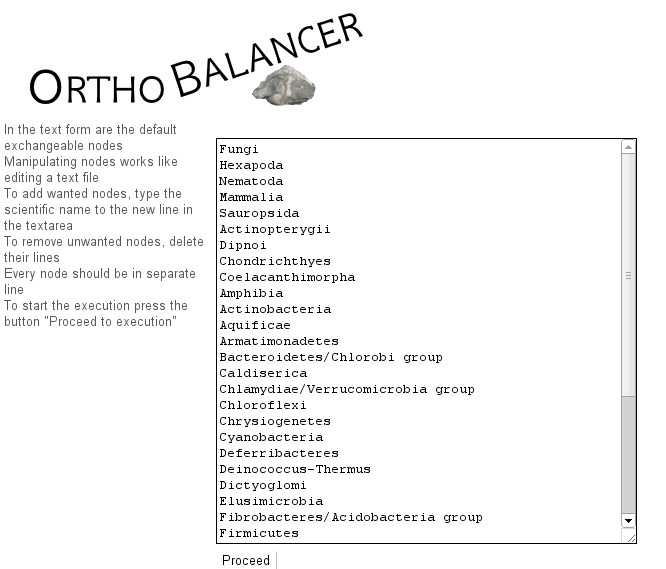
\includegraphics[width=5.0in]{figures/exchangeable-html.png}
\caption{Stranica za modificiranje zamjenskih čvorova}
\label{fig:exchangeable-html}
\end{figure} 
 
Ukoliko korisnik želi modificirati skup zamjenskih čvorova, umjesto pritiska na
gumb \emph{Proceed}, što odmah započinje pretragu, korisnik može pritisnuti gumb
\emph{Modify exchangeable nodes} na početnoj stranici. Time se otvara stranica
za modificiranje zamjenskih čvorova prikazana na slici
\ref{fig:exchangeable-html}. U području za unos teksta svaki redak sadrži
pojedini zamjenski čvor. Prilikom otvaranja navedene stranice u području se
nalazi predloženi skup čvorova koji se koristi i u pretrazi bez korisnikovog
modificiranja. Za korištenje funkcionalnosti podržane ovom stranicom preporučuje
se bolje poznavanje NCBI-jeve taksonomske baze.

\begin{figure}[h!]
\centering
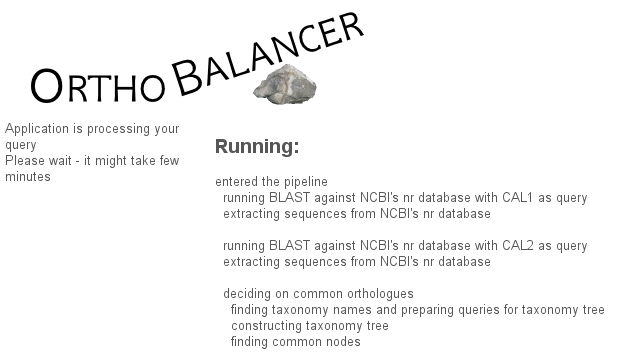
\includegraphics[width=5.0in]{figures/executing-html.png}
\caption{Stranica koja prikazuje tijek izvođenja}
\label{fig:executing-html}
\end{figure} 

Orthobalancer za vrijeme svog rada komunicira s prilično velikim bazama te
vrijeme izvođenja može potrajati nekoliko minuta. Kako je takvo ponašanje
očekivano, status izvođenja se prikazuje na stranici prikazanoj na slici
\ref{fig:executing-html}.
 
\begin{figure}[h!]
\centering
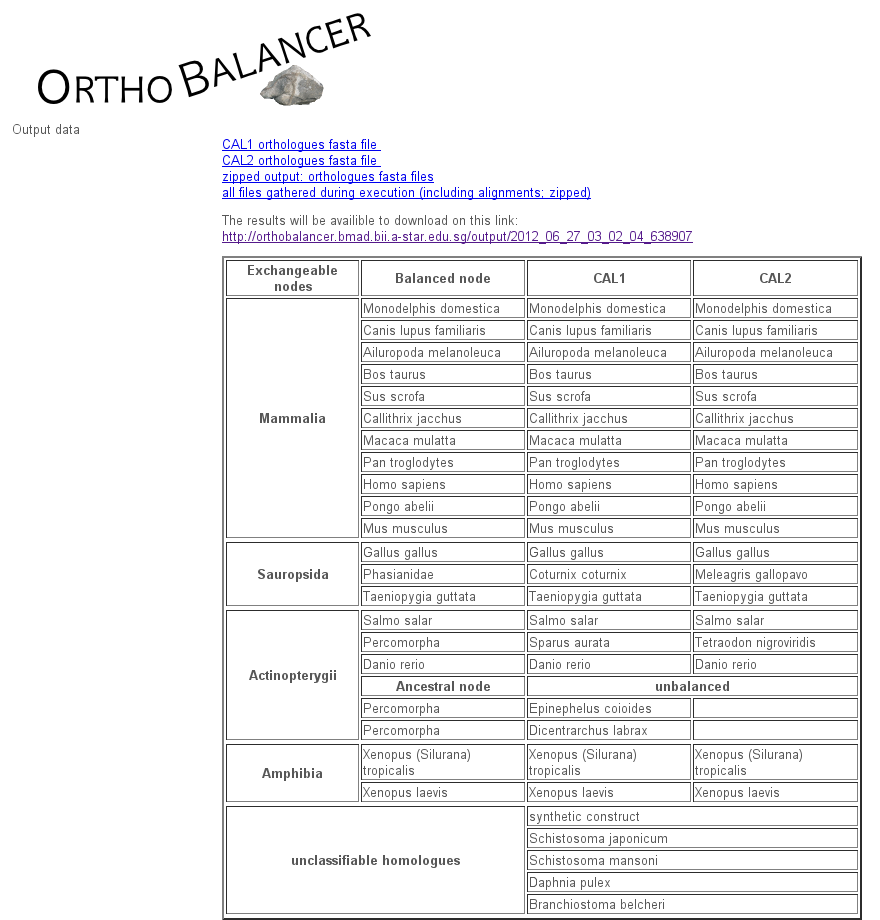
\includegraphics[width=5.8in]{figures/output-html.png}
\caption{Izlazna stranica}
\label{fig:output-html}
\end{figure} 
 
Završna stranica prikazana je na slici \ref{fig:output-html}. Na vrhu su
poveznice za preuzimanje izlaznih datoteka, a ispod njih se nalazi tablica
balansiranih vrsta. Tablica i datoteke su detaljnije objašnjeni u odjeljku
\ref{sec:output}.
